% ==============================================================================
% TCC - Nome do Aluno
% Capítulo 2 - Referencial Teórico
% ==============================================================================
\chapter{Algoritmo de Dijkstra}
\label{sec-dijkstra}

\section{O Algoritmo}
\label{sec-dijkstra-algoritmo}
O algoritmo de Dijkstra tem por objetivo definir o menor caminho partindo do vértice origem $v_{s}$ e chegando a todos os demais vértices $v_{i}$ do grafo $G = (V,E)$. Para garantir a viabilidade do algoritmo, assume-se que todos os pesos $w( u, v )$ sejam maiores ou iguais a zero para toda aresta $E$ do grafo $G$ \cite{cormen2009introduction}.

A seguir é apresentado o pseudocódigo do algoritmo conforme descrito em \citeonline{drozdek2012data}.
%\begin{verbatim}
%CÓDIGO AQUI
%\end{verbatim}

\begin{lstlisting}[ mathescape, label=lst-dijkstra-codigo, caption=Algoritmo de Dijkstra., float=htpb]
DijkstraAlgorithm(weighted simple digraph, vertex first)
	for all vertices v
		currDist(v) = $\infty$;
	currDist(first) = 0;
	toBeChecked = all vertices;
	while toBeChecked is not empty
		v = a vertex in toBeChecked with minimal currDist(v);
		remove v from toBeChecked;
		for all vertices u adjacent to v and in toBeChecked
			if currDist( u ) > currDist( v ) + weight( edge(vu) )
				currDist( u ) = currDist( v ) + weight( edge(vu) );
				predecessor( u ) = v;
\end{lstlisting}

%\begin{verbatim}
%DijkstraAlgorithm(weighted simple digraph, vertex first)
%	for all vertices v
%	currDist(v) = infinite;
%	currDist(first) = 0;
%	toBeChecked = all vertices;
%	while toBeChecked is not empty
%		v = a vertex in toBeChecked with minimal currDist(v);
%		remove v from toBeChecked;
%		for all vertices u adjacent to v and in toBeChecked
%		if currDist( u ) > currDist( v ) + weight( edge(vu) )
%			currDist( u ) = currDist( v ) + weight( edge(vu) );
%			predecessor( u ) = v;
%\end{verbatim}

O algoritmo inicia atribuindo o valor inicial de cada distância de cada vértice do grafo igual a $\infty$ com exceção do vértice inicial $v_{s}$ que será iniciado por 0. Em seguida todos os vértices são adicionados ao conjunto dos "toBeChecked" ("aSeremChecados"). Feito isso, inicia-se o processo iterativo: seleciona-se o vértice $v$ de menor custo que esteja dentro do conjunto "toBeChecked", retira-se ele do conjunto e a partir dele, para cada vértice adjacente $u$ de $v$, verifica-se se a distância atual calculada de $u$ é maior do que a distância calculada de $v$ mais o valor referente ao peso da aresta de $v$ e $u$ (origem em $v$). Caso seja verdade, a distância atual de $u$ é substituida pela soma da distância atual de $v$ mais o peso da aresta de $v$ e $u$ (este valor corresponde a distância do vértice de origem $v_{s}$ até $u$), além de definir o antecessor $u$ como sendo $v$. Repete-se o passo iterativo até que o conjunto "toBeChecked" esteja vazio.

Ao final do algoritmo, teremos o conjuto de predecessores de cada vértice do grafo, e a partir deste, poderemos definir a rota para qualquer vértice do grafo partindo de $v_{s}$.  %\footnote{Em liguagens de programação, é costume substituir este valor pelo maior número representativo do tipo da varíavel selecionado para representar a distância. Por exemplo na liguagem C, caso se utilize o valor int (inteiro) para representar a distância, a atribuição inicial será dado pela constante "int_max" definida na biblioteca "limits.h"}

\subsection{Garantia do algoritmo retorna o menor valor}
\label{sec-dijkstra-algoritmo-prova}
A prova será demonstrada em breve.

\section{Versões do Algoritmo implmentadas e suas Estrutura de Dados}
\label{sec-dijkstra-versoes}
Para este projeto de graduação, será implementada três versões do algoritmo de Dijkstra baseados em estruturas de dados diversas que implicam em tempos computacionais diferentes \cite{cormen2009introduction}.

As versões implementadas são o Dijkstra Canônico, Dijkstra Heap Binário (seção \ref{sec-dijkstra-versoes-heap}) e Dijkstra Heap de Fibonacci (seção \ref{sec-dijkstra-versoes-fibonacci}), todas baseadas em \citeonline{cormen2009introduction, drozdek2012data}.

Para a versão Dijkstra Canônico, o algoritmo utiliza de um vetor para armazenar as distâncias calculadas pelo algoritmo, e a cada passo iterativo (conforme demonstrado pelo algoritmo na seção \ref{sec-dijkstra-algoritmo}), uma busca linear é realizada para determinar o vértice fora do conjunto "toBeChecked", cuja a distância é menor dentre todas as outras. O tempo computacional para esse caso é $O(|V^{2}|)$ \cite{drozdek2012data}.

\subsection{Dijkstra Heap Binário}
\label{sec-dijkstra-versoes-heap}
Para esta implementação, será utilizada a estrutura de dados heap binária mínima como fila de prioridade. Heaps binária podem ser descritas como árvores binárias que possuem as seguintes propriedades \cite{drozdek2012data}:
\begin{enumerate}
 \item O valor de cada nodo não é maior do que os valores guardados em cada um de seus filhos.
 \item A árvore é perfeitamente balaceada, e as folhas no último nível estão todas mais a esquerda.
\end{enumerate}

Um exemplo de estrutura Heap Binário representada tanto como árvore como vetor pode ser visualizado nas figuras \ref{fig-dijkstra-heapbinario} e \ref{fig-dijkstra-heapvetor} respectivamente.

\begin{figure}[H]
\centering
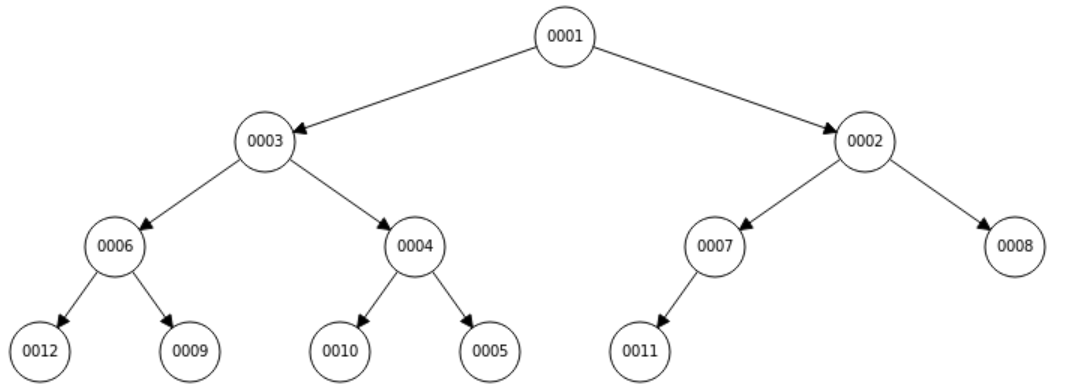
\includegraphics[width=.95\textwidth]{figuras/Heap} 
\caption{Exemplo de Heap Binário representado como árvore.}
\label{fig-dijkstra-heapbinario}
\end{figure}

\begin{figure}[H]
\centering
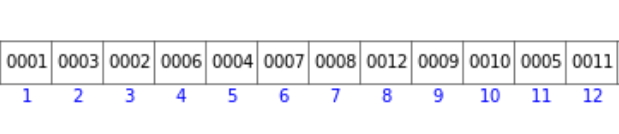
\includegraphics[width=.60\textwidth]{figuras/Heap-vetor}
\caption{Representação do Heap Binário da figura \ref{fig-dijkstra-heapbinario} como vetor.}
\label{fig-dijkstra-heapvetor}
\end{figure}

A vantagem de se usar essa estrutura de dados reside no fato de suas operações de inserção, extração de mínimo e reconstrução da heap possuirem tempo computacional de $O(\log n)$. Por consequência, o tempo computacional para este caso é de $O(|E| \log |V|)$ \cite{cormen2009introduction}.

\subsection{Dijkstra Heap de Fibonacci}
\label{sec-dijkstra-versoes-fibonacci}


\section{Experimentos Computacionais}
\label{sec-dijkstra-experimentos}


\section{Conclusões}
\label{sec-dijkstra-conclusoes}